% Goals
% Sie kennen das CLR Runtime System für .NET im Überblick
% Sie wissen was Assemblies sind und wie diese erstellt werden
% Sie kennen MSIL und verstehen den Vorgang der JIT-Kompilation
% Sie kennen das Common Type System mit Referenz- und Wertetypen
% Sie sind fähig, das .NET Command Line Interface CLI zu bedienen
% Sie verstehen, wie .NET-Projekte aufgebaut sind, wie diese Referenzen verwalten 
% Sie wissen, was NuGet Packages sind und wie diese eingesetzt werden können 
% Sie können erklären, für was .NET Standard Libraries verwendet werden sowie wann und wie sie eingesetzt werden

\section{Introduction}

\subsection{.NET Framework}
\begin{itemize}
  \itemsep 0em 
  \item Aktuellen werden über 30 Sprachen unterstützt
  \item Der Source Code wird in die Intermediate Language IL (ähnlich wie Assembler, vergleichbar mit Java Bytecode kopiert)
  \item Alle Sprachen nutzen das selbe Objektmodell und Bibliotheken
  	\SubItem{gemeinsamer IL-Zwischencode}
  	\SubItem{gemeinsames Typensystem (CTS)}
  	\SubItem{gemeinsame Runtime (CLR)}
  	\SubItem{gemeinsame Klassenbilbiotheken}
  	\SubItem{Das CLS definiert Einschränkungen an interoperablen Schnittstellen}
  \item Der Debugger unterstützt alle Sprachen (auch Cross-Language Debugging möglich)
\end{itemize}

\begin{figure}[h!]
	\centering
	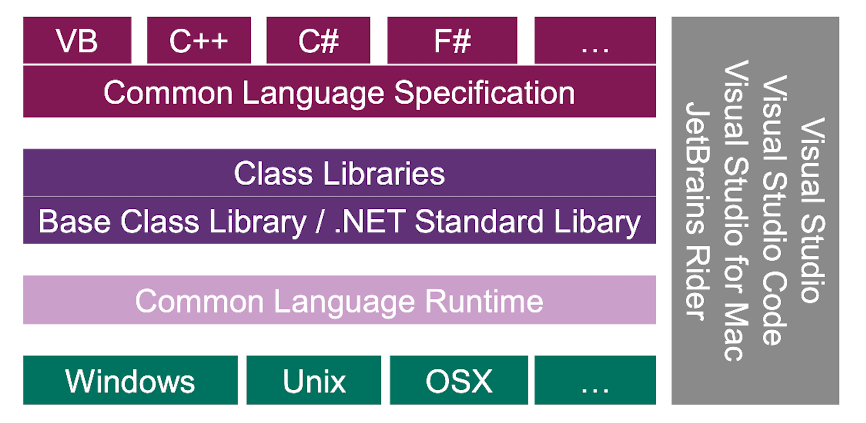
\includegraphics[width=0.5\textwidth]{framework}
    \caption{.NET Framework Architektur}
\end{figure}

\subsection{CLR: Common Language Runtime}
Die CLR ist die Laufzeitumgebung für .NET-Code und umfasst Funktionen wie: Just in Time Compilation etc. Man versteht unter dem CLR ein sprachunabhängiges, abstrahiertes Betriebssystem. Verantwortlichkeiten: Memory Management, Class Loading, Garbage Collection, Exceptions, Type Checking, Code Verification des IL-Codes, Debugging und Threading. Die CLR ist mit der Java VM vergleichbar.

\subsection{CTS: Common Type System}
Das allgemeine Typensystem legt fest, wie Typen in der Common Language Runtime deklariert, verwendet und verwaltet werden. Außerdem ist das System ein wichtiger Bestandteil der Laufzeitunterstützung für die sprachübergreifende Integration. Alle Typen in .NET sind entweder Werttypen oder Verweistypen. Alle Typen sind von System.Object abgeleitet. CTS ist teil der CLR.

\subsubsection{Reference- und Value Typen}
In .NET unterscheidet man zwischen Referenz- (Klassen) und Value Typen (Structs, Enum und primitive Datentypen).

\begin{minipage}{0,5\linewidth}
	\begin{itemize}
  		\itemsep -0.5em 
  		\item Reference Types
  			\SubItem{Werden auf dem Heap gespeichert}
  			\SubItem{Variable enthält Referenz}
  			\SubItem{Automatisch Garbage Collection}
  			\SubItem{Konstrutkor erzeugt und initialisiert Objekt}
  			\SubItem{Objekt hat eine Referenz auf seine Typenbeschreibung}
	\end{itemize}
	\centering
	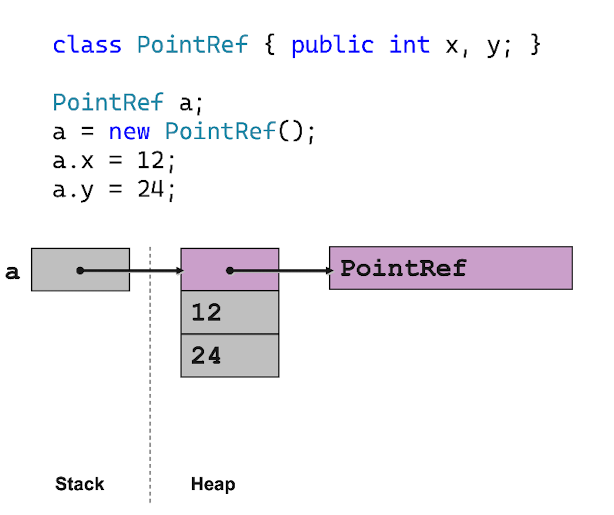
\includegraphics[width=0.75\linewidth]{referencetype}	
\end{minipage}
\begin{minipage}{0,5\linewidth}
	\begin{itemize}
  		\itemsep -0.5em 
  		\item Value Types
			\SubItem{Zur Speicherung Roher Werte auf dem Stack}
			\SubItem{Konstrutkor macht nur eine Initialisierung}
			\SubItem{Boxing: automatische Umwandlung von Reference Type}
			\SubItem{sealed}
	\end{itemize}
	\centering
	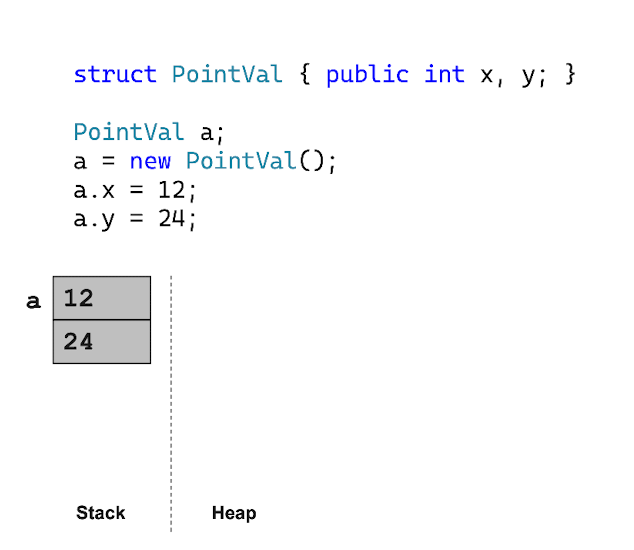
\includegraphics[width=0.75\linewidth]{valuetype}	  
\end{minipage}

\subsubsection{Boxing und Unboxing}
Boxing ermöglicht, dass Value- und Reference Types polymorph behandelt werden können. \textbf{Boxing:} Kopiert Value Type in einen Reference Type. Value Type wird implizit Konvertiert (UpCast). \textbf{Unboxing:} Kopiert Reference Type in eine Value Type. Explizite Konversion nötig!

\subsection{CLS: Common Language Specification}
 Um vollständige Interoperabilitätsszenarien zu aktivieren, müssen alle Objekte, die im Code erstellt werden, sich auf eine gewisse Gemeinsamkeit in den Sprachen verlassen, von denen sie verwendet werden (die ihre Aufrufer sind). Da es zahlreiche verschiedene Sprachen gibt, legt .NET diese Gemeinsamkeiten in der sogenannten Common Language Specification (CLS) fest. Die CLS definiert einen Satz von Funktionen, die viele gängige Anwendungen benötigen. Darüber hinaus bietet sie für jede Sprache, die in .NET implementiert wird, Anweisungen, was diese unterstützen muss. Die CLS ist eine Teilmenge des CTS.

\begin{figure}[h!]
	\centering
	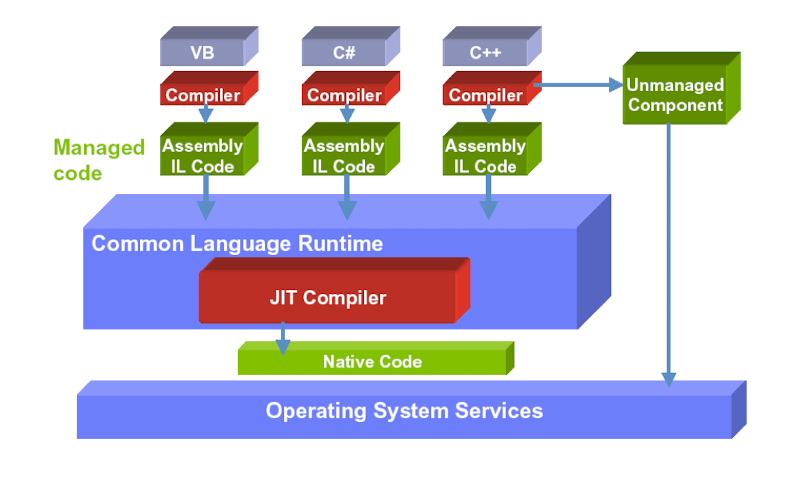
\includegraphics[width=0.6\textwidth]{clr}
    \caption{CLR: Common Language Runtime Architecture}
\end{figure}

\subsection{Microsoft Intermediate Language (MSIL)}
Die MSIL ist eine vorkompilierte Zwischensprache, welche: \textit{Prozessor-unabhängig, Assembler-ähnlich und Sprach-unabhängig ist.}

\begin{enumerate}
  \item Sprachspezifischer Kompilier kompiliert nach MSIL
  \item Just In Time Compiler (JIT) Compiler aus dem CLR kompiliert in nativen plattformabhängigen Code.
\end{enumerate}

\begin{itemize}
  \itemsep -0.5em 
  \item Vorteile
  \SubItem{Portabilität (Nicht-Intel-Prozessoren, Unix etc.)}
  \SubItem{Typensicherheit (Beim laden des Code können Typen- Sicherheit und weiter Security-Checks durchgeführt werden.}
  \item Nachteile
  \SubItem{Laufzeiteffizient (Kann durch den JIT-Compiler wettgemacht werden)}
\end{itemize}

\begin{figure}[h!]
	\centering
	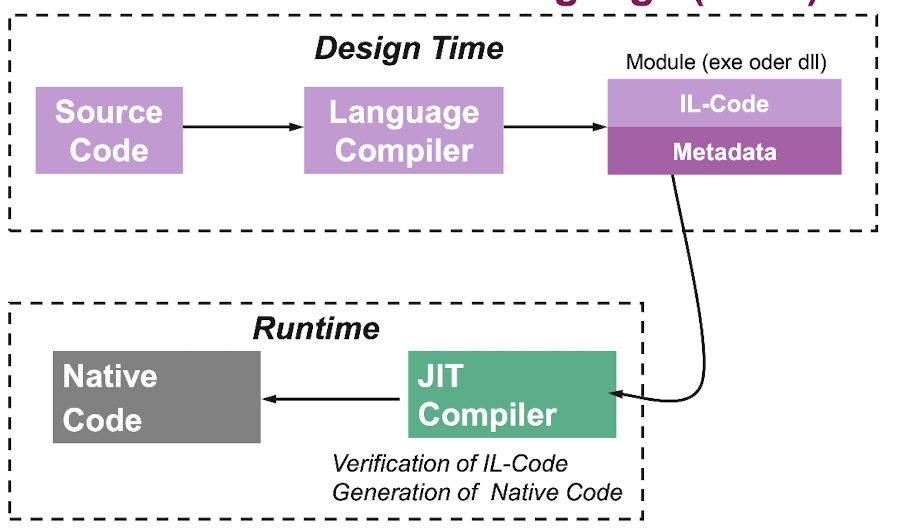
\includegraphics[width=0.5\textwidth]{msil}
    \caption{MSIL Kompilierung}
\end{figure}

\subsection{Assemblies}
Die Kompilation erzeugt Assemblies, welche mit einem JAR-File verglichen werden können. Assemblys sind ausführbare Dateien (.exe) oder Dynamic Link Library-Dateien (.dll) und bilden die Bausteine von .NET-Anwendungen. Sie stellen der Common Language Runtime die Informationen zur Verfügung, die sie zum Erkennen der Typenimplementierungen benötigt.

\begin{figure}[h!]
	\centering
  	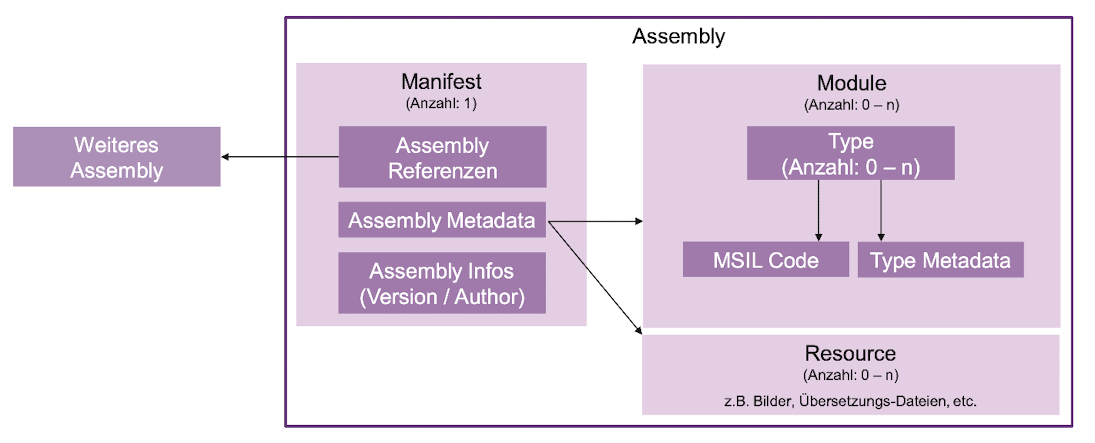
\includegraphics[width=0.75\textwidth]{assembly}
    \caption{Assembly Überblick}
\end{figure}

\subsubsection{Modules \& Metadata}
Eine Kompilation erzeugt ein Modul mit Code/MSIL und den Metadaten. Die Metadaten beschreiben alles Aspekte ausser die Programmlogik des Codes.

\pagebreak

\section{Projekte und Referenzen in Visual Studio}
Projekt-Dateien werden als XML-Datei verwaltet. Neu ist das *.csproj seit dem Jahre 2017.  Die Struktur ist identisch, wird aber anders interpretiert. Es gibt zwei Build Engines: Microsoft Build Engine (MSBuild) und .NET CORE CLI (dotnet build) - ist indirekt auch wieder MSBuild.

\subsection{Projektdateien}
Die neuen Projektdateien (*.csproj) sind viel Schlanker als die alten. Enthält neue Definition der vom Compiler unterstützen XML-Elemente und Attribute. 

\subsection{Referenzen}
Im Projektfile wird zwischen verschiednen Referenzen unterschieden.
\begin{itemize}
  \itemsep -0.5em 
  \item Vorkompiliertes Assembly
  	\SubItem{Im File System, Debugging nicht verfügbar, Navigation auf Metadaten-Ebene}
  \item NuGet Package
  	\SubItem{Externe Dependency, Debugging nicht verfügbar, Navigation auf Metadaten-Ebene}
  \item Visual Studio Projekt
  	\SubItem{In gleicher Solution vorhanden, Debugging und Navigation verfügbar}
  \item .NET Core oder .NET Standrad DSK
  	\SubItem{Zwingend, Normalerweise "Microsoft.NETCore.App", Bei .NET Standard "NETStandard.Library"}
\end{itemize}

\subsection{Packages \& NuGet}
.NET wird neu in kleineren NuGet Packages ausgeliefert und ist kein monolithisches Framework mehr. Vorteile: unterschiedliche Release-Zyklen, Erhöhte Kompatibilität, kleinere Deploymenteinheiten.

\pagebreak
